\documentclass[a4paper]{article}

\def\npart {III}
\def\nterm {Lent}
\def\nyear {2017}
\def\nlecturer {T. E. Forster}
\def\ncourse {Logic}
\def\nlectures {MWF.10}

% Imports
\ifx \nextra \undefined
  \usepackage[pdftex,
    hidelinks,
    pdfauthor={Dexter Chua},
    pdfsubject={Cambridge Maths Notes: Part \npart\ - \ncourse},
    pdftitle={Part \npart\ - \ncourse},
  pdfkeywords={Cambridge Mathematics Maths Math \npart\ \nterm\ \nyear\ \ncourse}]{hyperref}
  \title{Part \npart\ - \ncourse}
\else
  \usepackage[pdftex,
    hidelinks,
    pdfauthor={Dexter Chua},
    pdfsubject={Cambridge Maths Notes: Part \npart\ - \ncourse\ (\nextra)},
    pdftitle={Part \npart\ - \ncourse\ (\nextra)},
  pdfkeywords={Cambridge Mathematics Maths Math \npart\ \nterm\ \nyear\ \ncourse\ \nextra}]{hyperref}

  \title{Part \npart\ - \ncourse \\ {\Large \nextra}}
\fi

\author{Lectured by \nlecturer \\\small Notes taken by Dexter Chua}
\date{\nterm\ \nyear}

\usepackage{alltt}
\usepackage{amsfonts}
\usepackage{amsmath}
\usepackage{amssymb}
\usepackage{amsthm}
\usepackage{booktabs}
\usepackage{caption}
\usepackage{enumitem}
\usepackage{fancyhdr}
\usepackage{graphicx}
\usepackage{mathtools}
\usepackage{microtype}
\usepackage{multirow}
\usepackage{pdflscape}
\usepackage{pgfplots}
\usepackage{siunitx}
\usepackage{tabularx}
\usepackage{tikz}
\usepackage{tkz-euclide}
\usepackage[normalem]{ulem}
\usepackage[all]{xy}

\pgfplotsset{compat=1.12}

\pagestyle{fancyplain}
\lhead{\emph{\nouppercase{\leftmark}}}
\ifx \nextra \undefined
  \rhead{
    \ifnum\thepage=1
    \else
      \npart\ \ncourse
    \fi}
\else
  \rhead{
    \ifnum\thepage=1
    \else
      \npart\ \ncourse\ (\nextra)
    \fi}
\fi
\usetikzlibrary{arrows}
\usetikzlibrary{decorations.markings}
\usetikzlibrary{decorations.pathmorphing}
\usetikzlibrary{positioning}
\usetikzlibrary{fadings}
\usetikzlibrary{intersections}
\usetikzlibrary{cd}

\newcommand*{\Cdot}{\raisebox{-0.25ex}{\scalebox{1.5}{$\cdot$}}}
\newcommand {\pd}[2][ ]{
  \ifx #1 { }
    \frac{\partial}{\partial #2}
  \else
    \frac{\partial^{#1}}{\partial #2^{#1}}
  \fi
}

% Theorems
\theoremstyle{definition}
\newtheorem*{aim}{Aim}
\newtheorem*{axiom}{Axiom}
\newtheorem*{claim}{Claim}
\newtheorem*{cor}{Corollary}
\newtheorem*{defi}{Definition}
\newtheorem*{eg}{Example}
\newtheorem*{fact}{Fact}
\newtheorem*{law}{Law}
\newtheorem*{lemma}{Lemma}
\newtheorem*{notation}{Notation}
\newtheorem*{prop}{Proposition}
\newtheorem*{thm}{Theorem}

\renewcommand{\labelitemi}{--}
\renewcommand{\labelitemii}{$\circ$}
\renewcommand{\labelenumi}{(\roman{*})}

\let\stdsection\section
\renewcommand\section{\newpage\stdsection}

% Strike through
\def\st{\bgroup \ULdepth=-.55ex \ULset}

% Maths symbols
\newcommand{\bra}{\langle}
\newcommand{\ket}{\rangle}

\newcommand{\N}{\mathbb{N}}
\newcommand{\Z}{\mathbb{Z}}
\newcommand{\Q}{\mathbb{Q}}
\renewcommand{\H}{\mathbb{H}}
\newcommand{\R}{\mathbb{R}}
\newcommand{\C}{\mathbb{C}}
\newcommand{\Prob}{\mathbb{P}}
\renewcommand{\P}{\mathbb{P}}
\newcommand{\E}{\mathbb{E}}
\newcommand{\F}{\mathbb{F}}
\newcommand{\cU}{\mathcal{U}}
\newcommand{\RP}{\mathbb{RP}}
\newcommand{\CP}{\mathbb{CP}}

\newcommand{\ph}{\,\cdot\,}

\DeclareMathOperator{\sech}{sech}
\DeclareMathOperator{\cosech}{cosech}
\DeclareMathOperator{\cosec}{cosec}

\DeclareMathOperator{\covol}{covol}
\DeclareMathOperator{\vol}{vol}

\let\Im\relax
\let\Re\relax
\DeclareMathOperator{\Im}{Im}
\DeclareMathOperator{\Re}{Re}
\DeclareMathOperator{\im}{im}
\DeclareMathOperator{\image}{image}
\DeclareMathOperator{\Ann}{Ann}

\DeclareMathOperator*{\res}{res}
\DeclareMathOperator{\Res}{Res}
\DeclareMathOperator{\Ind}{Ind}

\DeclareMathOperator{\tr}{tr}
\DeclareMathOperator{\diag}{diag}
\DeclareMathOperator{\rank}{rank}
\DeclareMathOperator{\card}{card}
\DeclareMathOperator{\spn}{span}
\DeclareMathOperator{\adj}{adj}

\DeclareMathOperator{\erf}{erf}
\DeclareMathOperator{\erfc}{erfc}

\DeclareMathOperator{\ord}{ord}
\DeclareMathOperator{\Sym}{Sym}

\DeclareMathOperator{\sgn}{sgn}
\DeclareMathOperator{\orb}{orb}
\DeclareMathOperator{\stab}{stab}
\DeclareMathOperator{\ccl}{ccl}

\DeclareMathOperator{\lcm}{lcm}
\DeclareMathOperator{\hcf}{hcf}

\DeclareMathOperator{\Int}{Int}
\DeclareMathOperator{\id}{id}

\DeclareMathOperator{\betaD}{beta}
\DeclareMathOperator{\gammaD}{gamma}
\DeclareMathOperator{\Poisson}{Poisson}
\DeclareMathOperator{\binomial}{binomial}
\DeclareMathOperator{\multinomial}{multinomial}
\DeclareMathOperator{\Bernoulli}{Bernoulli}
\DeclareMathOperator{\like}{like}

\DeclareMathOperator{\var}{var}
\DeclareMathOperator{\cov}{cov}
\DeclareMathOperator{\bias}{bias}
\DeclareMathOperator{\mse}{mse}
\DeclareMathOperator{\corr}{corr}

\DeclareMathOperator{\otp}{otp}
\DeclareMathOperator{\dom}{dom}

\DeclareMathOperator{\Root}{Root}
\DeclareMathOperator{\supp}{supp}
\DeclareMathOperator{\rel}{rel}
\DeclareMathOperator{\Hom}{Hom}
\DeclareMathOperator{\Aut}{Aut}
\DeclareMathOperator{\Gal}{Gal}
\DeclareMathOperator{\Mat}{Mat}
\DeclareMathOperator{\End}{End}
\DeclareMathOperator{\Char}{char}
\DeclareMathOperator{\ev}{ev}
\DeclareMathOperator{\St}{St}
\DeclareMathOperator{\Lk}{Lk}
\DeclareMathOperator{\disc}{disc}
\DeclareMathOperator{\Isom}{Isom}
\DeclareMathOperator{\length}{length}
\DeclareMathOperator{\energy}{energy}
\DeclareMathOperator{\area}{area}
\DeclareMathOperator{\Syl}{Syl}
\DeclareMathOperator{\cl}{cl}
\DeclareMathOperator{\fix}{fix}

\newcommand{\GL}{\mathrm{GL}}
\newcommand{\SL}{\mathrm{SL}}
\newcommand{\PGL}{\mathrm{PGL}}
\newcommand{\PSL}{\mathrm{PSL}}
\newcommand{\PSU}{\mathrm{PSU}}
\newcommand{\Or}{\mathrm{O}}
\newcommand{\SO}{\mathrm{SO}}
\newcommand{\U}{\mathrm{U}}
\newcommand{\SU}{\mathrm{SU}}

\renewcommand{\d}{\mathrm{d}}
\newcommand{\D}{\mathrm{D}}

\tikzset{->/.style = {decoration={markings,
                                  mark=at position 1 with {\arrow[scale=2]{latex'}}},
                      postaction={decorate}}}
\tikzset{<-/.style = {decoration={markings,
                                  mark=at position 0 with {\arrowreversed[scale=2]{latex'}}},
                      postaction={decorate}}}
\tikzset{<->/.style = {decoration={markings,
                                   mark=at position 0 with {\arrowreversed[scale=2]{latex'}},
                                   mark=at position 1 with {\arrow[scale=2]{latex'}}},
                       postaction={decorate}}}
\tikzset{->-/.style = {decoration={markings,
                                   mark=at position #1 with {\arrow[scale=2]{latex'}}},
                       postaction={decorate}}}
\tikzset{-<-/.style = {decoration={markings,
                                   mark=at position #1 with {\arrowreversed[scale=2]{latex'}}},
                       postaction={decorate}}}

\tikzset{circ/.style = {fill, circle, inner sep = 0, minimum size = 3}}
\tikzset{mstate/.style={circle, draw, blue, text=black, minimum width=0.7cm}}

\definecolor{mblue}{rgb}{0.2, 0.3, 0.8}
\definecolor{morange}{rgb}{1, 0.5, 0}
\definecolor{mgreen}{rgb}{0.1, 0.4, 0.2}
\definecolor{mred}{rgb}{0.5, 0, 0}

\def\drawcirculararc(#1,#2)(#3,#4)(#5,#6){%
    \pgfmathsetmacro\cA{(#1*#1+#2*#2-#3*#3-#4*#4)/2}%
    \pgfmathsetmacro\cB{(#1*#1+#2*#2-#5*#5-#6*#6)/2}%
    \pgfmathsetmacro\cy{(\cB*(#1-#3)-\cA*(#1-#5))/%
                        ((#2-#6)*(#1-#3)-(#2-#4)*(#1-#5))}%
    \pgfmathsetmacro\cx{(\cA-\cy*(#2-#4))/(#1-#3)}%
    \pgfmathsetmacro\cr{sqrt((#1-\cx)*(#1-\cx)+(#2-\cy)*(#2-\cy))}%
    \pgfmathsetmacro\cA{atan2(#2-\cy,#1-\cx)}%
    \pgfmathsetmacro\cB{atan2(#6-\cy,#5-\cx)}%
    \pgfmathparse{\cB<\cA}%
    \ifnum\pgfmathresult=1
        \pgfmathsetmacro\cB{\cB+360}%
    \fi
    \draw (#1,#2) arc (\cA:\cB:\cr);%
}
\newcommand\getCoord[3]{\newdimen{#1}\newdimen{#2}\pgfextractx{#1}{\pgfpointanchor{#3}{center}}\pgfextracty{#2}{\pgfpointanchor{#3}{center}}}

\def\Xint#1{\mathchoice
   {\XXint\displaystyle\textstyle{#1}}%
   {\XXint\textstyle\scriptstyle{#1}}%
   {\XXint\scriptstyle\scriptscriptstyle{#1}}%
   {\XXint\scriptscriptstyle\scriptscriptstyle{#1}}%
   \!\int}
\def\XXint#1#2#3{{\setbox0=\hbox{$#1{#2#3}{\int}$}
     \vcenter{\hbox{$#2#3$}}\kern-.5\wd0}}
\def\ddashint{\Xint=}
\def\dashint{\Xint-}


\usepackage{bussproofs}
\newcommand\intro[1]{\RightLabel{\scriptsize#1-int}}
\newcommand\intron[2]{\RightLabel{\scriptsize#1-int (#2)}}
\newcommand\elim[1]{\RightLabel{\scriptsize#1-elim}}

\newenvironment{bprooftree}
  {\leavevmode\hbox\bgroup}
  {\DisplayProof\egroup}

\begin{document}
\maketitle
{\small
\setlength{\parindent}{0em}
\setlength{\parskip}{1em}
This course is the sequel to the Part II courses in Set Theory and Logic and in Automata and Formal Languages lectured in 2015-6. (It is already being referred to informally as ``Son of ST\&L and Automata \& Formal Languages''). Because of the advent of that second course this Part III course no longer covers elementary computability in the way that its predecessor (``Computability and Logic'') did, and this is reflected in the change in title. It will say less about Set Theory than one would expect from a course entitled `Logic'; this is because in Lent term Benedikt L\"owe will be lecturing a course entitled `Topics in Set Theory' and I do not wish to tread on his toes. Material likely to be covered include: advanced topics in first-order logic (Natural Deduction, Sequent Calculus, Cut-elimination, Interpolation, Skolemisation, Completeness and Undecidability of First-Order Logic, Curry-Howard, Possible world semantics, G\"odel's Negative Interpretation, Generalised quantifiers\ldots); Advanced Computability ($\lambda$-representability of computable functions, Tennenbaum's theorem, Friedberg-Muchnik, Baker-Gill-Solovay\ldots); Model theory background (ultraproducts, Los's theorem, elementary embeddings, omitting types, categoricity, saturation, Ehrenfeucht-Mostowski theorem\ldots); Logical combinatorics (Paris-Harrington, WQO and BQO theory at least as far as Kruskal's theorem on wellquasiorderings of trees\ldots). This is a new syllabus and may change in the coming months. It is entirely in order for students to contact the lecturer for updates.

\subsubsection*{Pre-requisites}
The obvious prerequisites from last year's Part II are Professor Johnstone's Set Theory and Logic and Dr Chiodo's Automata and Formal Languages, and I would like to assume that everybody coming to my lectures is on top of all the material lectured in those courses. This aspiration is less unreasonable than it may sound, since in 2016-7 both these courses are being lectured the term before this one, in Michaelmas; indeed supervisions for Part III students attending them can be arranged if needed: contact me or your director of studies. I am lecturing Part II Set Theory and Logic and I am even going to be issuing a ``Sheet 5'' for Set Theory and Logic, of material likely to be of interest to people who are thinking of pursuing this material at Part III. Attending these two Part II courses in Michaelmas is a course of action that may appeal particularly to students from outside Cambridge.
}
\tableofcontents

\section{Proof theory and constructive logic}
\subsection{Natural deduction}
The first person to have the notion of ``proof'' as a mathematical notion was probably G\"odel, and he needed this to write down the incompleteness theorem. The notion of proof he had was a very unintuitive notion. It is not very easy to manipulate, but they are easy to reason about.

In later years, people came up with more ``natural'' ways of defining proofs, and they are called natural deduction. In the formalism we learnt in IID Logic and Set Theory, we had three axioms only, and one rule of inference. In natural deduction, we have many rules of deduction.

We write or rules in the following form:
\[
  \begin{bprooftree}
    \AxiomC{$A$}
    \AxiomC{$B$}
    \intro{$\wedge$}
    \BinaryInfC{$A \wedge B$}
  \end{bprooftree}
\]
This says if we know $A$ and $B$ are true, then we can conclude $A \wedge B$. We call the things above the line the \term{premises}, and those below the line the \term{conclusions}. We can write out the other rules as follows:
\begin{center}
\begin{tabular}{cc}
   \begin{bprooftree}
    \AxiomC{$A$}
    \AxiomC{$B$}
    \intro{$\wedge$}
    \BinaryInfC{$A \wedge B$}
  \end{bprooftree} &
  \begin{bprooftree}
    \AxiomC{$A \wedge B$}
    \elim{$\wedge$}
    \UnaryInfC{$A$}
  \end{bprooftree}
  \begin{bprooftree}
    \AxiomC{$A \wedge B$}
    \elim{$\wedge$}
    \UnaryInfC{$B$}
  \end{bprooftree}\\[2em]
  \begin{bprooftree}
    \AxiomC{$A$}
    \intro{$\vee$}
    \UnaryInfC{$A \vee B$}
  \end{bprooftree}
  \begin{bprooftree}
    \AxiomC{$B$}
    \intro{$\vee$}
    \UnaryInfC{$A \vee B$}
  \end{bprooftree}\\[2em]
  &
  \begin{bprooftree}
    \AxiomC{$A$}
    \AxiomC{$A \to B$}
    \elim{$\to$}
    \BinaryInfC{$B$}
  \end{bprooftree}
\end{tabular}
\end{center}
Here we are separating these rules into two kinds --- the first column is the \term{introduction rules}. These tell us how we can \emph{introduce} a $\wedge$ or $\vee$ into our conclusions. The second column is the \term{elimination rules}. These tell us how we can \emph{eliminate} the $\wedge$ or $\to$ from our premises.

In general, we can think of these rules as ``LEGO pieces'', and we can use them to piece together to get ``LEGO assembles'', ie. proofs.
\begin{eg}
  For example, we might have a proof that looks like
  \begin{prooftree}
    \AxiomC{$A$}
    \intro{$\vee$}
    \UnaryInfC{$A \vee B$}
    \AxiomC{$A \vee B \to C$}
    \elim{$\to$}
    \BinaryInfC{$C$}
  \end{prooftree}
  This corresponds to a proof that we can prove $C$ from $A$ and $A \vee B \to C$. Note that sometimes we are lazy and don't specify the rules we are using.
\end{eg}
Instead of trying to formally describe how we can put these rules together to form a proof, we will work through some examples as we go, and it should become clear.

We see that we are missing some rules from the table, as there are no introduction rule for $\to$ and elimination rule for $\vee$.

We work with $\to$ first. How we can prove $A \to B$? To do so, we assume $A$, and then try to prove $B$. If we can do so, then we have proved $A \to B$. But we cannot express this in the form of our previous rules. Instead what we want is some ``function'' that takes proof trees to proof trees.

The actual rule is as follows: suppose we have derivation that looks like
\begin{prooftree}
  \AxiomC{$A$}
  \noLine
  \UnaryInfC{$\rvdots$}
  \noLine
  \UnaryInfC{$C$}
\end{prooftree}
This is a proof of C under the assumption A. The $\to$-introduction rule says we can take this and turn it into a proof of $A \to C$.
\begin{prooftree}
  \AxiomC{$\rvdots$}
  \noLine
  \UnaryInfC{$A \to C$}
\end{prooftree}
This rule is not a LEGO piece. Instead, it is a magic wand that turns a LEGO piece into a LEGO piece.

But we do not want magic wands in our proofs. We want to figure out some more static way of writing this rule. We decided that it should look like this:
\begin{prooftree}
  \AxiomC{$[A]$}
  \noLine
  \UnaryInfC{$\rvdots$}
  \noLine
  \UnaryInfC{$C$}
  \intro{$\to$}
  \UnaryInfC{$A \to C$}
\end{prooftree}
Here the brackets denotes that we have given up on our assumption $A$ to obtain the conclusion $A \to C$. After doing so, we are no longer assuming $A$. When we work with complicated proofs, it is easy to get lost where we are eliminating the assumptions. So we would label them, and write this as, say
\begin{prooftree}
  \AxiomC{$[A]^1$}
  \noLine
  \UnaryInfC{$\rvdots$}
  \noLine
  \UnaryInfC{$C$}
  \intron{$\to$}{1}
  \UnaryInfC{$A \to C$}
\end{prooftree}

\begin{eg}
  We can transform our previous example to say
  \begin{prooftree}
    \AxiomC{$[A]^1$}
    \intro{$\vee$}
    \UnaryInfC{$A \vee B$}
    \AxiomC{$A \vee B \to C$}
    \elim{$\to$}
    \BinaryInfC{$C$}
    \intron{$\to$}{1}
    \UnaryInfC{$A \to C$}
  \end{prooftree}
  Originally, we had a proof that $A$ and $A \vee B \to C$ proves $C$. Now what we have is a proof that $A \vee B \to C$ implies $A \to C$.
\end{eg}

Next, we need an elimination rule of $A \vee B$. What should this be? Suppose we proved \emph{both} that $A$ proves $C$, \emph{and} $B$ proves $C$. Then if we know $A \vee B$, then we know $C$ must be true.

In other words, if we have
\begin{prooftree}
  \AxiomC{$A \vee B$}
  \AxiomC{$A$}
  \noLine
  \UnaryInfC{$\rvdots$}
  \noLine
  \UnaryInfC{$C$}
  \AxiomC{$B$}
  \noLine
  \UnaryInfC{$\rvdots$}
  \noLine
  \UnaryInfC{$C$}
  \TrinaryInfC{}
\end{prooftree}
then we can deduce $C$. We write this as
\begin{prooftree}
  \AxiomC{$A \vee B$}
  \AxiomC{$[A]$}
  \noLine
  \UnaryInfC{$\rvdots$}
  \noLine
  \UnaryInfC{$C$}
  \AxiomC{$[B]$}
  \noLine
  \UnaryInfC{$\rvdots$}
  \noLine
  \UnaryInfC{$C$}
  \elim{$\vee$}
  \TrinaryInfC{$C$}
\end{prooftree}
There is an obvious generalization to many disjunctions:
\begin{prooftree}
  \AxiomC{$A_1 \vee \cdots\vee A_n$}
  \AxiomC{$[A_1]$}
  \noLine
  \UnaryInfC{$\rvdots$}
  \noLine
  \UnaryInfC{$C$}
  \AxiomC{$[A_n]$}
  \noLine
  \UnaryInfC{$\rvdots$}
  \noLine
  \UnaryInfC{$C$}
  \elim{$\vee$}
  \TrinaryInfC{$C$}
\end{prooftree}
How about when we have an empty disjunction? The empty disjunction is just false. So this gives the rule
\begin{prooftree}
  \AxiomC{$\bot$}
  \UnaryInfC{$B$}
\end{prooftree}
In other words, we can prove anything assume falsehood. This is known as \term{ex falso sequitur quolibet}.

Note that we did not provide any rules for talking about negation. We do not need to do so, because we just take $\neg A$ to be $A \to \bot$.

So far, what we have described it \term{constructive propositional logic}. What is missing? We cannot use our system to prove the \term{law of excluded middle}, $A \vee \neg A$, or the \term{law of double negation} $\neg \neg A \to A$. It is not difficult to convince ourselves that it is impossible to prove these using the laws we have described above.

To obtain \term{classical propositional logic}, we need just one more rule, which is
\begin{prooftree}
  \AxiomC{$[A\to \bot]$}
  \noLine
  \UnaryInfC{$\rvdots$}
  \noLine
  \UnaryInfC{$\bot$}
  \UnaryInfC{$A$}
\end{prooftree}
If we add this, then we get classical propositional calculus, and it is a theorem that any truth-table-tautology (ie. propositions that are always true for all possible values of $A, B, C$ etc) can be proved using natural deduction with the law of excluded middle.

\begin{eg}
  Suppose we want to prove
  \[
    A \to (B \to C) \to ((A \to B) \to (A \to C))
  \]
  How can we possibly prove this? The only way we can obtain this is to get something of the form
  \begin{prooftree}
    \AxiomC{$[A \to (B \to C)]$}
    \noLine
    \UnaryInfC{$\rvdots$}
    \noLine
    \UnaryInfC{$(A \to B) \to (A \to C)$}
    \intro{$\to$}
    \UnaryInfC{$A \to (B \to C) \to ((A \to B) \to (A \to C))$}
  \end{prooftree}
  Now the only way we can get the second-to-last conclusion is
  \begin{prooftree}
    \AxiomC{$A \to B$}
    \AxiomC{$[A]$}
    \noLine
    \BinaryInfC{$\rvdots$}
    \noLine
    \UnaryInfC{$C$}
    \UnaryInfC{$A \to C$}
  \end{prooftree}
  and then further eliminating $A \to B$ gives us $(A \to B) \to (A \to C)$. At this point we might see how we can patch them together to get a proof:
  \begin{prooftree}
    \AxiomC{$[A]^3$}
    \AxiomC{$[A \to (B \to C)]^1$}
    \BinaryInfC{$B \to C$}

    \AxiomC{$[A \to B]^2$}
    \AxiomC{$[A]^3$}
    \BinaryInfC{$B$}
    \BinaryInfC{$C$}
    \intron{$\to$}{3}
    \UnaryInfC{$A \to C$}
    \intron{$\to$}{2}
    \UnaryInfC{$(A \to B) \to (A \to C)$}
    \intron{$\to$}{1}
    \UnaryInfC{$A \to (B \to C) \to ((A \to B) \to (A \to C))$}
  \end{prooftree}
  Note that when we did $\to$-int (3), we consumed two copies of $A$ in one go. This is allowed, as an assumption doesn't become false after we use it once.

  However, some people study logical systems that do \emph{not} allow it, and demand that assumptions can only be used once. These are known as \term{resource logics}, one prominent example of which is \term{linear logic}.
\end{eg}

\begin{eg}
  Suppose we want to prove $A \to (B \to A)$. We have a proof tree
  \begin{prooftree}
    \AxiomC{$[A]^1$}
    \AxiomC{$[B]^2$}
    \BinaryInfC{$A$}
    \intron{$\to$}{2}
    \UnaryInfC{$B \to A$}
    \intron{$\to$}{1}
    \UnaryInfC{$A \to (B \to A)$}
  \end{prooftree}
  How did we manage to do the step from $A\;\; B$ to $A$? One can prove it as follows:
  \begin{prooftree}
    \AxiomC{$A$}
    \AxiomC{$B$}
    \intro{$\wedge$}
    \BinaryInfC{$A\wedge B$}
    \elim{$\wedge$}
    \UnaryInfC{$A$}
  \end{prooftree}
  but this is slightly unpleasant. It is redundant, and also breaks some nice properties of natural deduction we are going to prove later, eg. the subformula property. So instead, we just put an additional \term{weakening rule} that just says we can drop any assumptions we like at any time.
\end{eg}

\begin{eg}
  Suppose we wanted to prove
  \[
    A \to (B \wedge C) \to ((A \to B) \wedge (A \to C)).
  \]
  This is indeed a truth-table tautology, as we can write out the truth table and see this is always true.

  If we try very hard, we will find out that we cannot prove it without using the law of excluded middle. In fact, this is not valid in constructive logic. Intuitively, the reason is that assuming $A$ is true, which of $B$ or $C$ is true can depend on why $A$ is true, and this it is impossible to directly prove that either $A \to B$ is true, or $A \to C$ is true.

  Of course, this is true in classical logic.
\end{eg}

\begin{ex}
  Prove the following:
  \begin{itemize}
    \item $(P \to Q) \to ((Q \to R) \to (P \to R))$
    \item $(A \to C) \to ((A \wedge B) \to C)$
    \item $((A \vee B) \to C) \to (A \to C)$
    \item $P \to (\neg P \to Q)$
    \item $A \to (A \to A)$
    \item $(P \vee Q) \to ((( P \to R) \wedge (Q \to S)) \to R \vee S)$
    \item $(P \wedge Q) \to ((( P \to R) \vee (Q \to S)) \to R \vee S)$
    \item $A \to ((((A \to B) \to B) \to C) \to C)$
    \item $((((P \to Q) \to P) \to P ) \to Q) \to Q$
  \end{itemize}
  Don't do the last two.
\end{ex}

Instead of thinking of natural deduction as an actual logical theory, we often think of it as a ``platform'' that allows us to describe different logical theories, which we can do by introducing other connectives.

\begin{eg}
  For example, we might want to describe first-order logic. We can give introduction rules for $\exists$ as follows:
  \begin{prooftree}
    \AxiomC {$\varphi(t)$}
    \intro{$\exists$}
    \UnaryInfC{$\exists x\; \varphi(x)$}
  \end{prooftree}
  Similarly, we can have an elimination rule for $\forall$ easily:
  \begin{prooftree}
    \AxiomC{$\forall \varphi(x)$}
    \elim{$\forall$}
    \UnaryInfC{$\varphi(t)$}
  \end{prooftree}
  The introduction rule for $\forall$ is a bit more complicated. The rule again looks something like
  \begin{prooftree}
    \AxiomC {$\varphi(x)$}
    \intro{$\forall$}
    \UnaryInfC{$\forall x\; \varphi(x)$}
  \end{prooftree}
  but for such a proof to be valid, the $x$ must be ``arbitrary''. So we need an additional condition on this rule that there is no free occurence of $x$'s.

  Finally, suppose we know $\exists x\; \varphi(x)$. How can we use this to deduce some $p$? Suppose we know that $\varphi(x)$ implies $p$, and also $p$ does not depend on $x$. Then just knowing that there exists some $x$ such that $\varphi(x)$, we know $p$ must be true.
  \begin{prooftree}
    \AxiomC{$\exists x\; \varphi(x)$}
    \AxiomC{$\varphi(x)$}
    \noLine
    \UnaryInfC{$\rvdots$}
    \noLine
    \UnaryInfC{$p$}
    \elim{$\exists$}
    \BinaryInfC{$p$}
  \end{prooftree}
  Again we need $x$ to be arbitrary in $p$. % maybe clarify this more
\end{eg}

\begin{eg}
  We can also use natural deduction for ``naive set theory'', which we will later find to be inconsistent. We can give an $\in$-introduction rule
  \begin{prooftree}
    \AxiomC{$\varphi(x)$}
    \intro{$\in$}
    \UnaryInfC{$x \in \{y : \varphi(y)\}$}
  \end{prooftree}
  and a similar elimination rule
  \begin{prooftree}
    \AxiomC{$x \in \{y: \varphi (y)\}$}
    \elim{$\in$}
    \UnaryInfC{$\varphi(x)$}
  \end{prooftree}
\end{eg}

One cannot expect that we can write down whatever introduction and elimination rule we like, and expect to get a sensible theory. For example, if we introduce a connective $\&$ with the following silly rules:
\begin{center}
  \begin{bprooftree}
    \AxiomC{$A$}
    \intro{$\&$}
    \UnaryInfC{$A \& B$}
  \end{bprooftree}
  \begin{bprooftree}
    \AxiomC{$A \& B$}
    \elim{$\&$}
    \UnaryInfC{$B$}
  \end{bprooftree}
\end{center}
then this would immediately give us a theory that proves anything we like.

There are in fact two problems with our introduction and elimination rules. The first is that once we use our $A$ to deduce $A \& B$, it is completely gone, and we cannot recover anything about $A$ from $A \& B$. The second problem is that, obviously, proving $A \& B$ doesn't really involve $B$ at all, but we can use $A \& B$ to deduce something about $B$.

In general, to obtain a sensible natural deduction theory, we need harmony.
\begin{defi}[Harmony]\index{harmony}
  We say a connective $\$ $ is \term{harmonious} if $\phi \$ \psi$ is the strongest assertion you can deduce from the assumptions in the rule of $\$ $-introduction, and $\phi \$ \psi$ is the weakest thing that implies the conclusion of the $\$ $-elimination rule.
\end{defi}
We will not make the notion more precise than this.

\begin{eg}
  The introduction and elimination rules for $\in$ we presented are certainly harmonious, because the conclusions and assumptions are in fact equivalent.

  One can also check that the introduction and elimination rules for $\wedge$ and $\vee$ are harmonious.
\end{eg}

\begin{eg}[Russel's paradox]
  In naive set theory, consider
  \[
    R = \{x: x \in x \to \bot\}.
  \]
  Then we can have the deductions
  \begin{prooftree}
    \AxiomC{$R \to R$}
    \AxiomC{$R \to R$}
    \elim{$\in$}
    \UnaryInfC{$R \in R \to \bot$}
    \elim{$\to$}
    \BinaryInfC{$\bot$}
  \end{prooftree}
  We can then move on to use this to deduce that $R \in R$:
  \begin{prooftree}
    \AxiomC{$[R \to R]^1$}
    \AxiomC{$[R \to R]^1$}
    \elim{$\in$}
    \UnaryInfC{$R \in R \to \bot$}
    \elim{$\to$}
    \BinaryInfC{$\bot$}
    \intron{$\to$}{1}
    \UnaryInfC{$R \in R \to \bot$}
    \intro{$\in$}
    \UnaryInfC{$R \in R$}
  \end{prooftree}
  Now we have proved $R \in R$. But we previously had a proof that $R \in R$ gives a contradiction. So what we are going to do is to make two copies of this proof:
  \begin{prooftree}
    \AxiomC{$[R \to R]^1$}
    \AxiomC{$[R \to R]^1$}
    \elim{$\in$}
    \UnaryInfC{$R \in R \to \bot$}
    \elim{$\to$}
    \BinaryInfC{$\bot$}
    \intron{$\to$}{1}
    \UnaryInfC{$R \in R \to \bot$}
    \intro{$\in$}
    \UnaryInfC{$R \in R$}
    \AxiomC{$[R \to R]^2$}
    \AxiomC{$[R \to R]^2$}
    \elim{$\in$}
    \UnaryInfC{$R \in R \to \bot$}
    \elim{$\to$}
    \BinaryInfC{$\bot$}
    \intron{$\to$}{2}
    \UnaryInfC{$R \in R \to \bot$}
    \elim{$\to$}
    \BinaryInfC{$\bot$}
  \end{prooftree}
  So we showed that we have an inconsistent theory.

  Note that we didn't use a lot of ``logical power'' here. We didn't use the law of excluded middle, so this contradiction manifests itself even in the case of constructive logic. Moreover, we didn't really use many axioms of naive set theory. We didn't even need things like extensionality for this to work.
\end{eg}

Now we notice that this proof is rather weird. We first had an $\to$-introduction (2), and then subsequently eliminated it immediately. In general, if we have a derivation of the form
\begin{prooftree}
  \AxiomC{$P$}
  \noLine
  \UnaryInfC{$\rvdots$}
  \noLine
  \UnaryInfC{$Q$}
  \intro{$\to$}
  \UnaryInfC{$P \to Q$}
  \AxiomC{$\rvdots$}
  \noLine
  \UnaryInfC{$P$}
  \elim{$\to$}
  \BinaryInfC{$Q$}
\end{prooftree}
We can just move the second column to the top of the first to get
\begin{prooftree}
  \AxiomC{$\rvdots$}
  \noLine
  \UnaryInfC{$Q$}
\end{prooftree}

In general,
\begin{defi}[Maximal formula]\index{maximal formula}\index{formula}
  We say a formula in a derivation is \emph{maximal} iff it is both the conclusion of an occurence of an introduction rule, \emph{and} the major premiss of an occurnece of the elimination rule for the same connective.
\end{defi}

Here it is important that we are talking about the \emph{major} premise. In a deduction
\begin{prooftree}
  \AxiomC{$A \to B$}
  \AxiomC{$A$}
  \elim{$\to$}
  \BinaryInfC{$B$}
\end{prooftree}
we call $A \to B$ the \emph{major premise}, and $B$ the \emph{minor premise}. In the case of $\wedge$ and $\vee$, the terms are symmetric, and we do not need such a distinction.

This distinction is necessary since a deduction of the form
\begin{prooftree}
  \AxiomC{$(A \to B) \to C$}
  \AxiomC{$[A]$}
  \noLine
  \UnaryInfC{$\rvdots$}
  \noLine
  \UnaryInfC{$B$}
  \intro{$\to$}
  \UnaryInfC{$A \to B$}
  \elim{$\to$}
  \BinaryInfC{$C$}
\end{prooftree}

One can prove that any derivation in propositional logic can be converted to one that does not contain maximal formulae. However, if we try to eliminate the maximal fomrula in our proof of inconsistency of naive set theory, we will find that we will end up with the same proof!

\subsection{Curry--Howard correspondence}
Return to the days where we did IID Logic and Set Theory. Instead of natural deduction, we bootstrapped our system with two axioms $K$ and $S$:
\begin{itemize}
  \item[$K$:] $A\to(B\to A)$
  \item[$S$:] $[A\to(B\to C)]\to[(A\to B)\to(A \to C)]$
\end{itemize}
It is a fact that $\{K, S\}$ axiomatizes the conditional ($\to$) fragment of \emph{constructive} propositional logic. To axiomatize the conditional fragment of \emph{classical} logic, we need a new law, \term{Peirce's law}:
\[
  ((A \to B) \to A) \to A.
\]
In particular, we cannot prove Peirce's law from $K$ and $S$.

How can we go about proving that Peirce's law is unprovable? The most elementary way of doing so would be to try to allow for more truth values, such that $K$, $S$ and modus ponens hold, but Peirce's law does not. It turns out three truth values are sufficient. We consider the following truth table for $\to$:
\begin{center}
  \begin{tabular}{cccc}
    \toprule
    $\to$ & 1 & 2 & 3\\
    \midrule
    1 & 1 & 2 & 3\\
    2 & 1 & 1 & 3\\
    3 & 1 & 1 & 1\\
    \bottomrule
  \end{tabular}
\end{center}
Here we interpret $1$ as ``true'', $3$ as ``false'', and $2$ as ``maybe''.

By writing out the truth tables, one can verify that the formulas $K$ and $S$ always take truth value $1$. Also, if $A$ and $A \to B$ are both $1$, then so is $B$. So by induction on the structure of the proof, we know that anything deduced from $K$ and $S$ and \emph{modus ponens} will have truth value $1$.

However, if we put $A = 2$ and $B = 3$, then $((A \to B) \to A) \to A$ has value $2$, not $1$. So it cannot possibly be deduced from $K$ and $S$.

This is, of course, a very unsatisfactory answer. The truth table was just pulled out of a hat, and we just checked to see that Peirce's law doesn't hold. It doesn't tell us where the truth table came from, and \emph{why} we can't prove Peirce's law.

We will answer the second question first using the \emph{Curry--Howard correspondence}. Then we will see how we can come up with this truth table using \emph{possible world semantics} in the next chapter.

Consider the piece of syntax
\[
  A \to B.
\]
So far, we have viewed this as a logical formula --- $A$ and $B$ are formulae, and $\to$ denotes implication. However, in mathematics, there is another common use of this notation --- we can think of $A$ and $B$ as sets, and $A \to B$ is the set of all functions from $A$ to $B$. The idea of the Curry--Howard correspondence is to view implication as functions between sets.

While this might seem like a bizarre thing to do, it actually makes sense. Given a formula $A$, we can view $A$ as a ``set'', whose ``elements'' are the proofs of $A$. Now if we know $A \to B$, this means any proof of $A$ becomes a proof of $B$. In other words, we have a function $A \to B$. As we move on, we will see that this idea of viewing a formula $A$ as the set of all proofs of $A$ gives a very close correspondence between the logical connectives and set-theoretic constructions.

This is also known as \term{propositions as types}, and it is common to call $A$, $B$ etc ``types'' instead of ``sets''.

Under this correspondence, \emph{modus ponens} has a very natural interpretation. We can just think of the rule
\begin{prooftree}
  \AxiomC{$A$}
  \AxiomC{$A \to B$}
  \BinaryInfC{$B$}
\end{prooftree}
as function application! If we have an element $a\in A$, and an element $f \in A \to B$, then we have $f(a) \in B$. Now it is awkward to write $f \in A \to B$ instead of $f: A \to B$. So in fact, we will write $f: A \to B$ instead. Moreover, we will use the colon instead of $\in$ for \emph{all} types. So we can write
\begin{prooftree}
  \AxiomC{$x: A$}
  \AxiomC{$f: A \to B$}
  \BinaryInfC{$f(x): B$}
\end{prooftree}
Often, we will just write $fx$ instead of $f(x)$. If we write $fxy$, then it means $(fx)y$, but we will usually put brackets to indicate.

\begin{eg}
  What is the interpretation of $K$ under the Curry--Howard correspondence? It corresponds to a function
  \[
    A \to (B \to A).
  \]
  Let's try to think of a function that does this. Given an element $a: A$, we need to find a function $B \to A$. Since the only thing we know about is $a$, we could return the constant function that always returns $a$. So for each $a : A$, we define $K(a)$ to be the constant function $a$.

  This is indeed where the name $K$ came from. It's just that the inventor was German, and so it is not $C$.
\end{eg}
What about conjunction? To prove $A \wedge B$, we need to prove $A$ and $B$. In other words, an element of $A \wedge B$ should be an element of the Cartesian product $A \times B$.

We can write the introduction rule as
\begin{prooftree}
  \AxiomC{$x: A$}
  \AxiomC{$y: B$}
  \BinaryInfC{$\bra x, y\ket: A \wedge B$}
\end{prooftree}
Here we are using the angled brackets to denote ordered pairs. The elimination rules are just given by the projection $\fst: A \times B \to A$ and $\snd: A \times B \to B$:
\begin{center}
  \begin{bprooftree}
    \AxiomC{$x: A \wedge B$}
    \UnaryInfC{$\fst(x): A$}
  \end{bprooftree}
  \begin{bprooftree}
    \AxiomC{$x: A \wedge B$}
    \UnaryInfC{$\snd(x): B$}
  \end{bprooftree}
\end{center}
Some people write $\fst$ and $\snd$ as $\pi_1$ and $\pi_2$ instead.

We are not going to talk about the rules for ``or'', because they are horrendous. But if we think hard about it, then $A \vee B$ corresponds to the disjoint union of $A$ and $B$. % include

So far, we only know how to decorate our LEGO pieces. When we assemble them to get proofs, we can get more complicated tress. Suppose we had the tree
\begin{prooftree}
  \AxiomC{$[A \wedge B]^1$}
  \elim{$\wedge$}
  \UnaryInfC{$B$}
  \AxiomC{$[A \wedge B]^1$}
  \elim{$\wedge$}
  \UnaryInfC{$A$}
  \intro{$\wedge$}
  \BinaryInfC{$B \wedge A$}
  \intron{$\to$}{1}
  \UnaryInfC{$(A \wedge B) \to (B \wedge A)$}
\end{prooftree}
We now try to decorate this tree:
\begin{prooftree}
  \AxiomC{$x: [A \wedge B]^1$}
  \elim{$\wedge$}
  \UnaryInfC{$\snd(x): B$}
  \AxiomC{$x: [A \wedge B]^1$}
  \elim{$\wedge$}
  \UnaryInfC{$\fst(x): A$}
  \intro{$\wedge$}
  \BinaryInfC{$\bra \snd(x), \fst(x)\ket : B \wedge A$}
  \intron{$\to$}{1}
  \UnaryInfC{$(A \wedge B) \to (B \wedge A)$}
\end{prooftree}
Note that both $[A \wedge B]^1$ are decorated using the same letter $x$. This is since they are cancelled at the same time, so we are using the same instance of $A \wedge B$ in the statement $(A \wedge B) \to (B \wedge A)$.

Now the remaining question to answer is how we are going to decorate the $\to$-introduction. We want some notation that denotes the function that takes $x$ and returns $\bra \snd(x), \fst(x)$. More generally, if we have an expression $\varphi(x)$ in $x$, we want a notation that denotes the function that takes in $x$ and returns $\varphi(x)$.

The convention is to denote this using a $\lambda$:\index{$\lambda$}
\[
  \lambda x. \varphi(x).
\]
These expressions we produce are known as \term{$\lambda$ expressions}\index{lambda expressions}.

For example, in the previous case, the final result is
\[
  \lambda x. \bra \fst(x), \snd(x)\ket : (A \wedge B) \to (B \wedge A).
\]
The general decoration rule for $\to$-introduction is
\begin{prooftree}
  \AxiomC{$x: [A]^1$}
  \noLine
  \UnaryInfC{$\rvdots$}
  \noLine
  \UnaryInfC{$\varphi(x): C$}
  \intron{$\to$}{1}
  \UnaryInfC{$\lambda x. \varphi(x): A \to C$}
\end{prooftree}
Recall that previously we had a rule for getting rid of maximal formulae. Given a tree of the form
\begin{prooftree}
  \AxiomC{$P$}
  \noLine
  \UnaryInfC{$\rvdots$}
  \noLine
  \UnaryInfC{$Q$}
  \intro{$\to$}
  \UnaryInfC{$P \to Q$}
  \AxiomC{$\rvdots$}
  \noLine
  \UnaryInfC{$P$}
  \elim{$\to$}
  \BinaryInfC{$Q$}
\end{prooftree}
We can just move the second column to the top of the first to get
\begin{prooftree}
  \AxiomC{$\rvdots$}
  \noLine
  \UnaryInfC{$Q$}
\end{prooftree}
This conversion corresponds to the conversion
\[
  (\lambda x. \varphi(x)) a \rightsquigarrow \varphi(a),
\]
which is just applying the function! This process is known as \term{$\beta$-reduction}\index{beta-reduction}.

Since there is $\beta$-reduction, there is, of course, also \term{$\alpha$-reduction}\index{alpha-reduction}-reduction, but this is boring. It is just re-lettering $\lambda x. \phi(x)$ to $\lambda y. \phi(y)$. There will also be an $\eta$-reduction, and we will talk about that later.

In the following exercise/example, note that we have a convention that if we write $A \to B \to C$, then we mean $A \to (B \to C)$.
\begin{ex}
  Find $\lambda$-expressions that encode proofs of
  \begin{enumerate}
    \item $((A \to B) \wedge (C \to D)) \to ((A \wedge C) \to (B \wedge D))$
    \item $(A \to B) \to (B \to C) \to (A \to C)$ % insert convention about associativity somewhere
    \item $((A \to B) \to A) \to (A \to B) \to B$
    \item $(A \to B \to C) \to (B \to A \to C)$
    \item $(A \to B \to C) \to ((A \wedge B) \to C)$
    \item $(B \wedge A \to C) \to (A \to B \to C)$
  \end{enumerate}
\end{ex}

\begin{proof}[Solutions]\leavevmode
  \begin{enumerate}
    \item $\lambda f. \lambda x. \bra \fst(f)(\fst(x)), \snd(f)(\snd(x))\ket$
    \item $\lambda f. \lambda g. \lambda a. g(fa)$
    \item $\lambda f. \lambda g. g(fg)$
    \item $\lambda f. \lambda b. \lambda a. (fa)b$
    \item $\lambda f. \lambda x. f(\fst x)(\snd x)$
    \item $\lambda f. \lambda a. \lambda b. f\bra b, a\ket$
  \end{enumerate}
  One can write out the corresponding trees explicitly. For example, (iii) can be done by
  \begin{prooftree}
    \AxiomC{$g: [A \to B]^1$}
    \AxiomC{$f: [(A \to B) \to A]^2$}
    \elim{$\to$}
    \BinaryInfC{$fg: A$}
    \AxiomC{$g: [A \to B]^1$}
    \elim{$\to$}
    \BinaryInfC{$g(fg)$}
    \intron{$\to$}{1}
    \UnaryInfC{$\lambda g. g(fg): (A \to B) \to B$}
    \intron{$\to$}{2}
    \UnaryInfC{$\lambda f. \lambda g. g(fg): (A \to B) \to A \to (A \to B) \to B$}
  \end{prooftree}
  Note that we always decorate assumptions with a single variable, say $f$, even if they are very complicated. For example, if we have an assumption $A \wedge B$, it might be tempting to decorate it as $\bra a, b\ket$, but we do not.
\end{proof}

Now what we have is that for any proof tree, we obtain a $\lambda$ formula. But for any formula, it can have many proofs, and so it can be given by many $\lambda$ formula.
\begin{eg}
  Consider
  \begin{prooftree}
    \AxiomC{$x: [A]^1$}
    \AxiomC{$f: [A \to A]^2$}
    \elim{$\to$}
    \BinaryInfC{$fx: A$}
    \intron{$\to$}{1}
    \UnaryInfC{$\lambda x. fx: A \to A$}
    \intron{$\to$}{2}
    \UnaryInfC{$\lambda f. \lambda x. fx: (A \to A) \to (A \to A)$}
  \end{prooftree}
  This is really just the identity function!

  We can also try something slightly more complicated.
  \begin{prooftree}
    \AxiomC{$x: [A]^1$}
    \AxiomC{$f: [A \to A]^2$}
    \BinaryInfC{$f x: A$}
    \AxiomC{$f: [A \to A]^2$}
    \BinaryInfC{$f(f x): A$}
    \intron{$\to$}{1}
    \UnaryInfC{$\lambda x. f(f(x)): A \to A$}
    \intron{$\to$}{2}
    \UnaryInfC{$\lambda f. \lambda x. f(f x): (A \to A) \to (A \to A)$}
  \end{prooftree}
  This is another $\lambda$ term for $(A \to A) \to (A \to A)$. This says given any $f$, we return the function that does $f$ twice. These are two genuinely different functions, and thus these two $\lambda$ terms correspond to two different \emph{proofs} of $(A \to A) \to (A \to A)$.
\end{eg}

Note that given any proof tree, we can produce some $\lambda$ expression representing the proof rather systematically. However, given any $\lambda$ expression, it is difficult to figure out what it is a proof of, or if it represents a proof at all. For example, if we write down
\[
  \lambda x. xx,
\]
then we have no idea what this can possibly mean.

The problem is that we don't know what formula, or \emph{type} each variable is representing. The expression
\[
  \lambda f. \lambda x. f (f x)
\]
is confusing, because we need to guess that $x$ is probably just some arbitrary variable of type $A$, and that $f$ is probably a function $A \to A$. Instead, we can make these types explicit:
\[
  \lambda f_{A \to A}. \lambda x_A. f_{A \to A} (f_{A \to A} x_A).
\]
Given such a term, we can systematically deduce that it is of type $(A \to A) \to (A \to A)$, ie. it encodes a proof of $(A \to A) \to (A \to A)$. Such an expression with explicit types is known as a \term{typed $\lambda$ term}\index{typed lambda term}, and one without types is known as an \term{untyped $\lambda$ term}\index{untyped lambda term}.

Moreover, it is also straightforward to reconstruct the proof tree from this expression. Of course, we need to make sure the typing of the expression is valid. For example, we cannot write
\[
  f_{A \to A} x_B,
\]
since $f$ is not a function from $B$. Assuming we restrict to these valid terms, we have established a correspondence
\begin{significant}
  Proofs in propositional natural deduction are in a $1$-to-$1$ correspondence with typed $\lambda$ terms.
\end{significant}
That is, if we also make it clear what the rules for $\vee$ are.

Finally, what about $\bot$? To what set does the proposition $\bot$ correspond? The proposition $\bot$ should have \emph{no} proofs. So we would think $\bot$ should correspond to $\emptyset$.

In propositional calculus, the defining property of $\bot$ is that we can prove any proposition we like from $\bot$. Indeed, the empty set is a set that admits a function to any set $X$ whatsoever, and in fact this function can be uniformly defined for all sets, by the empty function. We again see that the ideas of propositional calculus correspond nicely with the properties of sets.

\begin{eg}
  Consider the law of excluded middle:
  \[
    ((A \to \bot) \to \bot) \to A.
  \]
  Can we write down a $\lambda$ expressions for this?

  We will argue rather informally. If there is a $\lambda$ expression of this type, then it should define the function ``uniformly'' without regards to what $A$ is about. We now see what this function could be.
  \begin{itemize}
    \item If $A$ is empty, then $A \to \bot$ contains exactly the empty function. So $(A\to \bot) \to \bot$ is the empty set, since there is no function from a non-empty set to the empty set. And there is a function $\emptyset \to A$, namely the empty function again.
    \item If $A$ is non-empty, then $A \to \bot$ contains no functions, so $(A \to \bot) \to \bot$ contains the empty function. So $((A \to \bot) \to \bot) \to A$ is given by exactly an element of $A$.
  \end{itemize}
  We see that to construct such a function, we need to first know if $A$ is empty or not. If it is non-empty, then we have to arbitrarily pick an element of $A$. Thus, there is no way we can uniformly construct such a function without knowing anything about $A$.
\end{eg}

\begin{prop}
  We cannot prove $((A \to B) \to A) \to A$ in natural deduction without the law of excluded middle.
\end{prop}

\begin{proof}
  Suppose there were a lambda term of type $((A \to B) \to A) \to A$.

  We pick
  \[
    B = \{0, 1\}, \quad A = \{0, 1, 2, 3, 4\}.
  \]
  In this setting, any function $f: A \to B$ identifies a distinguished member of $B$, namely the one that is hit by more members of $A$. We know $B \subseteq A$, so this is an element in $A$. So we have a function $(A \to B) \to A$. If we really had a lambda term $((A \to B) \to A) \to A$, then it would give us a member of $A$.

  % to be completed later
\end{proof}

\subsection{Possible world semantics}
For classical logic, semantics was easy. We had a collection of propositions $P$, and a model is just a function $P \to \{\top, \bot\}$. We can then define truth in this model recursively in the obvious way.

It turns out to get a sensible model theory of constructive logic, we need to consider \emph{many} such objects.

\begin{defi}[Possible world semantics]\index{possible world semantics}
  Let $P$ be a collection of propositions. A \term{world}\index{possible world semantics!world} is a subset $w \subseteq P$. A \term{model}\index{possible world semantics!model} is a collection $W$ of worlds, and a partial order $\geq$ on $W$ called \term{accessibility}\index{possible world semantics!accessibility}, satisfying the \term{persistence}\index{possible world semantics!persistence} property:
  \begin{itemize}
    \item If $p \in P$ is such that $p \in w$ and $w' \geq w$, then $p \in w'$.
  \end{itemize}
  Given any proposition $\varphi$, we define the relation $w \vDash \varphi$ by
  \begin{itemize}
    \item $w \not\vDash \bot$
    \item If $\varphi$ is \emph{atomic} (and not $\bot$), then then $w \vDash \varphi$ iff $\varphi \in w$.
    \item $w \vDash \varphi \wedge \psi$ iff $w \vDash \varphi$ and $w \vDash \psi$.
    \item $w \vDash \varphi \vee \psi$ iff $w \vDash \varphi$ or $w \vDash \psi$.
    \item $w \vDash \varphi \to \psi$ iff (for all $w' \geq w$, if $w' \vDash \varphi$, then $w' \vDash \psi$).
  \end{itemize}
  We will say that $w$ ``believes'' $\varphi$ if $w \vDash \varphi$, and that $w$ ``sees'' $w'$ if $w'' \geq w$.

  We also require that there is a designated minimum element under $\leq$, known as the \term{root world}. We can think of a possible world model as a poset decorated with worlds, and such a poset is called a \term{frame}. % replace poset with quasi-order, remove comment later on
\end{defi}
All but the last rule are obvious. The idea is that each world can have some beliefs, namely the subset $w \subseteq p$. The important idea is that if a world $w$ does not believe in $p$, it does not mean it believes that $p$ is false. It just that $w$ remains ignorant about whether $p$ is true.

Now we have $w' \geq w$ if $w'$ a more knowledgable version of $w$ that has more beliefs. Alternatively, $w'$ is a world whose beliefs are compatible with that of $w$. It is easy to show by induction that if $\varphi$ is \emph{any formula} that $w$ believes, and $w' \geq w$, then $w'$ also believes in $\varphi$. Then we can interpret the law of implication as saying ``$w$ believes that $p \to q$ iff for any possible thinkable world where $p$ is true, then $q$ is also true''.

Note that if we only have one world, then we recover models of classical logic.

What happens to negation? By definition, we have $w \vDash \neg A$ iff $w \vDash A \to \bot$. Expanding the definition, believing that $\neg A$ means there is no possible world compatible with $w$ in which $A$ is true. This is much stronger than just saying $w \not\vDash A$, which just says we do not hold any opinion on whether $A$ is true.

\begin{eg}
  We want to construct a world $w$ where $w \not \vDash A\vee \neg A$. So we need a $W$ such that $w$ neither believes $A$ nor believes $\neg A$.

  We can achieve the former by just making the world not believe in $A$. To make the world not believe $\neg A$, it needs to be able to see a world $w'$ such that $w' \vDash A$. So we can consider the following world:
  \begin{center}
    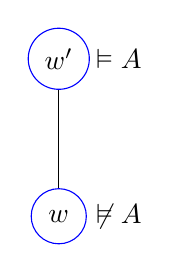
\begin{tikzpicture}
      \node [mstate] (1) at (0, 0) {$w'$};
      \node [right=10pt] at (1) {$\vDash A$};

      \node [mstate] (2) at (0, -2) {$w$};
      \node [right=10pt] at (2) {$\not\vDash A$};

      \draw (1) edge (2);
    \end{tikzpicture}
  \end{center}
\end{eg}

\begin{eg}
  This time consider the statement $w \vDash \neg \neg A \to A$. This takes some work to unravel.

  We need a world $w$ such that for all $w' \geq w$, if $w' \vDash \neg \neg A$, then $w' \vDash A$. If we unravel a bit more, we find that $w' \vDash \neg \neg A$ means for any $w'' \geq w'$, we can find some $w''' \geq w''$ such that $w''' \vDash A$.

  It is easy to see that actually in the model of the previous question, $w \not\vDash \neg \neg A \to A$, since $w \vDash \neg \neg A$, but $w \not\vDash A$.
\end{eg}

\begin{eg}
  The following model is a counter-model for $\neg \neg A \vee \neg A$:
  \begin{center}
    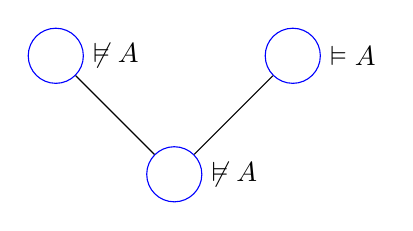
\begin{tikzpicture}
      \node [mstate] (b) at (0, 0) {};
      \node [right=10pt] at (b) {$\not\vDash A$};

      \node [mstate, above right=of b] (r) {};
      \node [right=10pt] at (r) {$\vDash A$};

      \node [mstate, above left=of b] (l) {};
      \node [right=10pt] at (l) {$\not\vDash A$};

      \draw (b) edge (r);
      \draw (b) edge (l);
    \end{tikzpicture}
  \end{center}
  where the bottom world believes in neither $\neg \neg A$ nor $\neg A$, since it sees worlds where $\neg A$ is true and also worlds where $A$ is true.
\end{eg}

Usually, we don't talk about a particular world believing in something. We talk about an entire structure of possible worlds believing something.
\begin{notation}
  If the root world of our model is $w$, then we write
  \[
    \vDash \varphi \Longleftrightarrow w \vDash \varphi.
  \]
\end{notation}
Almost by definition, if $\vDash \varphi$, then for any world $w'$, we have $w' \vDash \varphi$.

\begin{ex}
  Find a possible world model that does not believe Peirce's law.
\end{ex}

One can readily verify that classically, we have $(A \to B) \to B$ is equivalent to $A \vee B$, but they are not constructively equivalent.
\begin{ex}
  Find a possible world model that $\vDash (A \to B) \to B$, but does not $\vDash A \vee B$.
\end{ex}

\begin{ex}
  Find a possible world model that $\vDash (A \to B) \to B$ but does not believe $\vDash (B \to A) \to A$.
\end{ex}

\begin{ex}
  Find a possible world model that does not believe in $\vDash (A \to B) \vee (B \to A)$.
\end{ex}

Possible world semantics can be used for all sorts of logical systems, not just propositional logic. In general, the notion of accessibility need not be a partial order, but can be anything we want. Also, we do not necessarily have to require persistence. Of course, we also need to modify the according notion of a world.

\begin{eg}
  If we want to produce possible world semantics for constructive first-order logic, we need to modify our definition of worlds so that they have ``elements''. Assuming we have done so, we can encode $\forall$ and $\exists$ using the following rules:
  \begin{itemize}
    \item $w \vDash \exists x, F(x)$ if there is some $y \in w$ for which $w \vDash F(y)$.
    \item $w \vDash \forall x, F(x)$ if for all $w' \geq w$ and $x \in w'$, we have $w' \vDash F(x)$.
  \end{itemize}
  The second condition is much stronger than the naive ``for all $x \in w$, we have $w \vDash F(x)$'', because the $w'' \geq w$ may have many more elements. What our condition say is that $w$ somehow has a ``global'' way of showing that everything satisfies $F$.
\end{eg}

Let's talk a bit about persistence of formulae. We $\varphi$ is persistent iff $w \vDash\varphi$, $w' \geq w$ implies $w' \vDash \varphi$. By definition, all atomic formulae are persistent by stipulation. We can prove by induction that all formulae are persistent. This is just a massive yet easy proof by cases, and we will not do so.

\begin{eg}
  The proposition $A \to \neg \neg A$ is valid all possible world models.

  % To see this, we note that if we have a world $w$ that believes in $A$, then by persistence, any world that $A$ sees also believes in $A$. We want to show that it does not believe in $\neg A$. % complete proof, make use of reflexivity and transitivity
\end{eg}

% insert talk about finiteness of possible world models, therefore decidable.

Now suppose we have a possible world model in front of us. Then given a formula $\varphi$, the set of worlds that believe $\varphi$ is an upward-closed subset of the frame. So we can think of the truth value of $\varphi$ as these upward-closed set.
\begin{eg}
  Suppose we have the following worlds:
  \begin{center}
    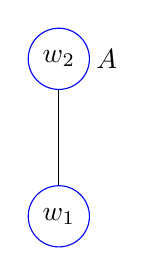
\begin{tikzpicture}
      \node [mstate] (1) at (0, 0) {$w_2$};
      \node [right=10pt] at (1) {$A$};

      \node [mstate] (2) at (0, -2) {$w_1$};

      \draw (1) edge (2);
    \end{tikzpicture}
  \end{center}
  So the top world only believes $A$, and the root world doesn't believe anything. The possible truth values are
  \[
    \emptyset, \{w_2\}, \{w_1, w_2\}.
  \]
  This is indeed the three-valued algebra we used to disprove Peirce's law. % check
\end{eg}
What can we say about the collection of upward-closed subset of frames, ie. our truth values? Under inclusion, it is easy to see that these are complete and co-complete, ie. we have all infinite unions and intersections.
\begin{defi}[Heyting algebra]\index{Heyting algebra}
  A Heyting algebra is a complete poset with joins $\wedge$ and $\vee$ and an operator $\to$ such that $A \Rightarrow B$ is the largest $C$ such that
  \[
    C \wedge A \leq B.
  \]
\end{defi}
We would expect
\[
  A \Rightarrow B = \vee \{C : C \wedge A \leq B\}.
\]
The only thing we need to check is that this choice of $A \Rightarrow B$ does indeed satisfy $(A \Rightarrow B) \wedge A \leq B$. % fix this!

The thought is that Heyting algebras would ``validate'' all constructive theses, by interpreting $\wedge$ with $\wedge$, $\vee$ with $\vee$ and $\rightarrow$ with $\Rightarrow$.

In other words, if we try to build a truth table for a formula with values in a Heyting algebra, we will get the top element $\top$ all the time iff the formula is constructively valid. So we have a parallel between the relation between classical logic and boolean algebras, and constructive logic and Heyting algebras.

Note that in classical logic, we only ever use the two-element boolean algebra. If we use the 4-element Boolean algebra, then we would detect the same set of tautologies. However, in the case of constructive logic we genuinely need all Heyting algebras.

\begin{lemma}
  Any formula with a natural deduction proof not using the rule for classical negation is true in all possible world models.
\end{lemma}
For any frame $F$, every such formula is satisfied by every possible world model on that frame. We say it is \emph{valid on $F$}. Such formulae are valid on all quasi-ordered sets with a bottom element.

\begin{proof}
  The hard case is implication. Suppose we have a natural deduction proof of $A \to B$. The last rule is a $\to$-introduction. So by the induction hypothesis, every world that believes $A$ also believes $B$. Now let $w$ be a world that believes all the other undischarged assumptions in $A \to B$. By persistence, every $w' \geq w$ believes similarly. So any $w' \geq w$ that believes $A$ also believes $B$. So $w \vDash A \to B$.
\end{proof}

\subsection{Negative interpretation}
Suppose a constructive logician found a classical logician, and then they try to talk to each other. Then they would find that they disagree on a lot of things. The classical logician has no problems accepting $\neg \neg A \to A$, but the constructive logician thinks that is nonsense. Can they make sense of each other?

The classical logician can understand the constructive logician via possible world semantics. He could think that when the constructive logician says a proposition is false, they mean there are possible world models where the proposition fails. This is all fine.

But can a constructive logician make sense of the classical logician? When the constructivist sees $A \vee B$, he thinks that either we can prove $A$, or we can prove $B$. However, the classical logician views this as a much weaker statement. It is more a long the lines of ``it is not true that $A$ and $B$ are both false''. In general, we can try to interpret classical statements by putting in enough negations:
\begin{center}
  \begin{tabular}{cc}
    \toprule
    Classical proposition & Constructive interpretation\\
    \midrule
    $A \vee B$ & $\neg (\neg A \vee \neg B)$\\
    $A \wedge B$& $A \wedge B$\\
    $\exists x\; W(x)$ & $\neg \forall x \neg W(x)$\\
    $A \to B$ & $\neg (A \wedge \neg B)$\\
    \bottomrule
  \end{tabular}
\end{center}
This gives rise to the \emph{negative interpretation} of classical logic into constructive logic, due to G\"odel:
\begin{defi}[Negative interpretation]\index{negative interpretation}
  Given a proposition $\phi$, the interpretation $\phi^*$ is defined recursively by
  \begin{itemize}
    \item $\bot^* = \bot$.
    \item If $\varphi$ is atomic, then $\varphi^* = \neg\neg \varphi$.
    \item If $\varphi$ is negatomic, then $\varphi^* = \varphi$.
    \item If $\varphi = \psi \wedge \theta$, then $\varphi^* = \psi^* \wedge \theta^*$.
    \item If $\varphi = \psi \vee \theta$, then $\varphi^* = \neg (\neg \psi^* \wedge \neg \theta^*)$.
    \item If $\varphi = \forall x\; \psi(x)$, then $(\forall x)(\psi^*(x))$.
    \item If $\varphi = \psi \to \theta$, then $\varphi^* = \neg(\psi^* \wedge \neg \theta^*)$.
    \item If $\varphi = \exists \; \psi(x)$, then $\varphi^* = \neg \forall x \neg \psi^*(x)$.
  \end{itemize}
\end{defi}
One can check that we always have $\vdash \varphi \to \varphi^*$. So the constructive version is always stronger.

\begin{defi}[Stable formula]\index{stable formula}
  A formula is \emph{stable} if
  \[
    \vdash \varphi^* \to \varphi.
  \]
\end{defi}

\begin{lemma}
  Any formula built up from negated and doubly negated atomics by $\neg$, $\wedge$ and $\forall$ is stable.
\end{lemma}

\begin{proof}
  By induction on formulae. The base case is immediate, using the fact that $\neg \neg \neg A \to \neg A$. More generally, we have
  \[
    (((p \to q) \to q) \to q) \to p \to q.
  \]
  It is less confusing to prove this in two steps, and we will write $\lambda$-terms for our proofs. First note that if we have $f: A \to B$, then we can obtain $f^T: (B \to q) \to A \to q$ for any $q$,  using
  \[
    f^T = \lambda g_{B \to q}. \lambda a_A: g(f(a)).
  \]
  So it suffices to prove that
  \[
    p \to (p \to q) \to q,
  \]
  and the corresponding term is
  \[
    \lambda x_p. \lambda g_{p \to q}. g x
  \]
  We now proceed by induction.
  \begin{itemize}
    \item Now assume that we have proofs of $\neg \neg p \to p$ and $\neg \neg q \to q$. We want to prove $p \wedge q$ from $\neg \neg (p \wedge q)$. It suffices to prove $\neg \neg p$ and $\neg \neg q$ form $\neg \neg (p \wedge q)$, and we will just do the first one by symmetry.

      We suppose $\neg p$. Then we know $\neg (p \wedge q)$. But we know $\neg \neg (p \wedge q)$. So we obtain a contradiction. So we have proved that $\neg \neg p$.
    \item Note that we have
      \[
        \vdash \exists x \neg \neg \varphi(x) \to \neg \neg \exists x \varphi(x),
      \]
      but not the other way round. For universal quantification, we have
      \[
        \neg \neg \forall x \varphi(x) \to \forall x \neg \neg \varphi(x),
      \]
      but not the other way round. We can construct a proof as follows:
      \begin{prooftree}
        \AxiomC{$[\forall x) \varphi(x)]^1$}
        \elim{$\forall$}
        \UnaryInfC{$\varphi(a)$}
        \AxiomC{$[\neg \varphi(x)]^2$}
        \elim{$\to$}
        \BinaryInfC{$\to$}
        \intron{$\to$}{1}
        \UnaryInfC{$\neg \forall x \varphi(x)$}
        \AxiomC{$[\neg \neg \forall x \varphi(x)]^3$}
        \elim{$\to$}
        \BinaryInfC{$\bot$}
        \intron{$\to$}{2}
        \UnaryInfC{$\neg \neg \varphi(a)$}
        \intro{$\forall$}
        \UnaryInfC{$\neg \neg \forall \varphi(x)$}
        \intron{$\to$}{3}
        \UnaryInfC{$\neg \neg \forall x F(x) \to \forall x \neg \neg F(x)$}
      \end{prooftree}
      We now want to show that if $\varphi$ is stable, then $\forall x \varphi(x)$ is stable. In other words, we want
      \[
        \neg \neg \forall x \varphi^*(x) \to \forall x \varphi^*(x).
      \]
      But form $\neg \neg \forall x \varphi^*(x)$, we can deduce $\forall x \neg \neg \varphi^*(x)$, which implies $\forall x \varphi^* (x)$.
  \end{itemize}
  So every formula in the range of the negative interpretation is stable. Every stable formula is equivalent to its double negation (classically). Every formula is classically equivalent to a stable formula.
\end{proof}
So if a constructive logician meets a classical logician who is making some bizarre assertions about first order logic. To make sense of this, the constructive logician can translate it to its negative interpretation, which the classical logician thinks is equivalent to the original one. And now these interpretations follow the law of excluded middle.

\subsection{Constructive mathematics}
We now want to try to do mathematics constructively. We note that even classically, if we do not have the law of excluded middle, then we have many distinct notions of ``finite set''. When we go constructive, things get more complicated.

We look at several possible definitions of finite sets.
\begin{defi}[Kuratowski finite]\index{Kuratowski finite}\index{finite!Kuratowski}
  We define ``finite'' recursively: $\emptyset$ is Kuratowski finite. If $x$ is Kuratowski finite, then so is $x \cup \{y\}$.
\end{defi}

There is a separate definition of $N$-finiteness:
\begin{defi}[$N$-finite]\index{$N$-finite}\index{finite!$N$}
  $\emptyset$ is $N$-finite. If $x$ is $N$-finite, and $y \not \in x$, then $x \cup \{y\}$ is $N$-finite.
\end{defi}
These two definitions are not the same! In a $N$-finite set, we know any two things are either equal, or they are not, as this is built into the definition of an $N$-finite set. However, in the case of Kuratowski finite, this is not true, since we don't have the law of exlcuded middle. We say $N$-finite sets have \term{decidable equality}.
If we want to do constructive arithmetic, the correct notion is $N$-finiteness.

We can still define natural numbers as the smallest set containing $\emptyset$ and is closed under successor. This gives us $N$-finite sets, but the least number principle is dodgy. It turns out the least number principle implies excluded middle.

It is helpful to note the following two definitions:
\begin{defi}[Non-empty set]\index{non-empty set}
  A set $x$ is non-empty if $\neg (\forall y)(y \not \in x)$.
\end{defi}

\begin{defi}[Inhabited set]\index{inhabited set}
  A set $x$ is inhabited if $(\exists y)(y \in x)$.
\end{defi}
\printindex
\end{document}
